\documentclass[prl,twocolumn,floatfix]{revtex4-2}

\usepackage{graphicx}
\usepackage{bm}

\usepackage{amsmath}
\usepackage{units}

\usepackage{hyperref}
\hypersetup{colorlinks=true, citecolor=blue, urlcolor=blue, linkcolor=blue}

\usepackage{todonotes}

\renewcommand{\vec}[1]{\boldsymbol{#1}}
\newcommand{\com}[1]{{\color{magenta} #1}}
\newcommand{\rework}[1]{{\color{blue}{#1}}}


\begin{document}
\title{Magnetic dichroism in darkfield UV photoemission electron microscopy}
\author{Maximilian Paleschke$^{1}$, David Huber$^{1}$, Friederike Wührl$^1$, Cheng-Tien Chiang$^2$, Frank O. Schumann$^3$, Jürgen Henk$^1$, Wolf Widdra$^1$}

\affiliation{$^1$Institute of Physics, Martin Luther University Halle-Wittenberg, D-06099 Halle (Saale), Germany}

\affiliation{$^2$Institute of Atomic and Molecular Sciences, Academia Sinica, Taipei, Taiwan}

\affiliation{$^3$Max-Planck-Institut f\"{u}r Mikrostrukturphysik, 06120 Halle, Germany}

\email{wolf.widdra@physik.uni-halle.de}

\date{\today}

\begin{abstract}
    Photoemission electron microscopy (PEEM) has evolved into an indispensable tool for structural and magnetic characterization of surfaces at the nanometer scale. Particularly, synchrotron-radiation-based X-ray PEEM has emerged as a leading method for probing element-specific magnetic properties via magnetic circular dichroism (MCD) in core level photoemission. In laboratory settings, UV radiation is utilized for near-threshold PEEM, which, when combined with femtosecond lasers, offers the potential for ultrafast time resolution. However, the characterization of magnetic properties, such as local magnetic domain structures, has seen limited application in UV-PEEM, with studies reporting only weak magnetic dichroism effects for in-plane magnetization. 
    Here we introduce the concept of darkfield PEEM for MCD in threshold photoemission. This method enables efficient MCD imaging with a significantly enhanced MCD contrast—by an order of magnitude—for in-plane magnetization, as demonstrated for Fe(001). This advancement paves the way for MCD imaging on femtosecond timescales using modern lasers. Darkfield PEEM imaging employs an aperture for photoelectron momentum selection in the back focal plane of the electron imaging column before forming the real-space image. While the general momentum dependence of the MCD contrast will be explained through symmetry considerations, the experimental results for Fe(001) will be quantitatively compared with state-of-the-art full-relativistic photoemission calculations.
\end{abstract}

\pacs{}

\maketitle
% Paragraph headings may be deleted in the final version .
\paragraph{Introduction.} Ultrafast spin and magnetization dynamics are exciting and rapidly growing fields in condensed matter physics with promising implications for both future research and device applications. Ultrafast imaging of magnetic domains on the micrometer scale is well established based on all-optical methods, as e.g. Kerr microscopy. On the nanometer scale, however, electron microscopy is the method of choice due to electrons short de Broglie wavelength. 
For imaging magnetic domains the magnetic circular dichroism (MCD) contrast is used in photoelectron emission microscopy (PEEM). The intensity recorded for a particular domain changes with the helicity of the incident radiation, thereby producing magnetic contrast without the need for an explicit electron spin detection. By tuning the incident X-ray radiation to a magnetic core level absorption edge, substantial and element-specific MCD asymmetries have been reported. With the wide availability of tunable synchrotron radiation, this technique of XMCD-PEEM is well established for magnetic domain imaging on the nanometer scale and for slow dynamics \cite{kuch15}. However, the pulse length of synchrotron radiation of typically 30-50 ps renders XMCD-PEEM unsuitable on ultrafast timescales. 
Replacing the incident X-ray radiation by ultrashort laser pulses solves this issue straightforwardly and allows for pump-probe experiments on a few femtoseconds timescale. In addition, experiments can be performed in the laboratory with UV laser sources, which excite electrons close to the Fermi level to energies slightly above the escape threshold. However, the reported MCD contrasts are quit small in threshold photoemission, especially for in-plane magnetization. 

As we demonstrate here, the concept of darkfield PEEM in threshold photoemission allows efficient MCD imaging with an order-of-magnitude enhanced MCD contrast for in-plane magnetization. It paves the way for MCD imaging on femtosecond timescales with modern UV laser sources.
Darkfield PEEM imaging uses an aperture for photoelectron momentum selection in the back focal plane of the electron imaging column prior to forming the real space image. We will demonstrate this for the in-plane magnetic structure at the Fe(001) surface and  compare quantitatively the experimental results with state-of-the-art full-relativistic photoemission calculations.

\todo[inline]{Check review of existing literature below} Following the initial reports of magnetic dichroism in UV photoemission and its theoretical description in 1991 and 1996 \cite{schneider1991,henk1996,feder1996}, Marx \textit{et al.}\ reported the first observation of magnetic dichroism in threshold PEEM in 2000 \cite{marx2000}. This study on polycrystalline Fe revealed a linear asymmetry of 0.37\,\%. 
Subsequent spectroscopic studies confirmed the presence of both circular and linear dichroism in various ferromagnetic materials. Building on Marx's experimental work, Nakagawa \textit{et al.}\ examined Ni films adsorbed with Cs, discovering significant asymmetries up to 12\,\% in circular dichroism PEEM for out-of-plane oriented domains \cite{nakagawa2007,nakagawa2009,nakagawa2012}. This work also demonstrated the feasibility of using pulsed laser light for dichroism imaging. However, due to the limited photon energy of common optical laser setups, Cs remains necessary in most photoemission experiments to reduce the work function \cite{kronseder2011, meier2017}. For instance, investigations of domains on the FePt surface employed a pulsed deep-UV laser with a photon energy of 7\,eV \cite{zhao2019}. 
The theoretical framework for valence-band dichroism was primarily developed in the 1990s and early 2000s by Feder, Henk, Kuch, Schneider, and Venus \cite{feder1996,henk1996,kuch1996a,kuch2001,venus1994,venus1997}, and was bolstered by pioneering experiments conducted by Tamura, Schmiedekamp, Kirschner, and Hild \cite{tamura1987, schmiedeskamp1988, venus95, hild2008, hild2009, hild2010}. It is based on calculating the relativistic band structure in conjunction with a theoretical description of the photoemission process. \todo[inline]{Do we need to cite Getzlaff'22 \cite{getzlaff2022}?}
\begin{figure}
    \centering
    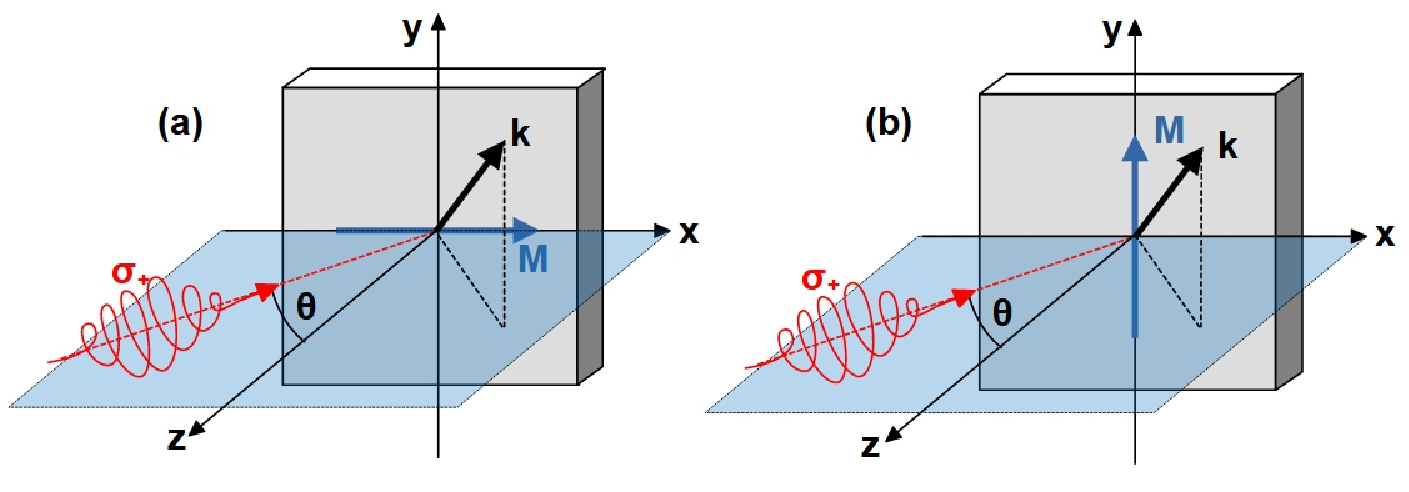
\includegraphics[width = \columnwidth]{symmetry}
    \caption{Symmetry analysis. A circular polarized laser pulse (orange, with helicity $\sigma_{+}$ impinges onto a magnetic domain (rectangular solid). The light incidence direction and the surface normal ($z$-axis) span the scattering plane (blue; $xz$-plane) with magnetization direction $\vec{M}$ oriented within or perpendicular to the scattering plane in (a) and (b), respectively. Note that the off-normal detection of photoelectrons with wavevector $\vec{k}$ (black arrow) results in a chiral setup. 
    % \rework{If the scattering plane is a mirror plane of the lattice, the photoemission intensities for fixed $\vec{k}$ obey $I(\sigma_{+}, +\vec{M}) = I(\sigma_{-}, -\vec{M})$ (panel~a) or $I(\sigma_{+}, +\vec{M}) = I(\sigma_{-}, +\vec{M})$ (panel~b).}
    }
    \label{fig:symmetry}
    % \todo[inline]{Should we exchange the figure by normal incidence and electron in scattering plane?}
\end{figure}




\paragraph{Conceptual basis.} For a simplified conceptual approach we consider a surface with fourfold symmetry, as e.g. the (001) fcc or bcc surfaces with magnetic easy axes along the four [100] directions. Let's assume light incidence along the surface normal (Fig.~\ref{fig:symmetry} for $\theta=0$). The photoemission intensity of electrons detected with off-normal wavevector $\vec{k}$ depends then on the helicity, $\sigma_{+}$ or $\sigma_{-}$, of the incident circular polarized laser radiation and on the two orientations $\pm M$ of the in-plane magnetization in a selected domain, yielding four intensities $I_{\vec{k}}(\sigma_{\pm}, \pm M)$ (shortened $I_{\pm \pm}$). The latter intensities are combined into the total intensity
\begin{align}
    I & \equiv I_{+ +} + I_{+ -} + I_{- +} + I_{- -}. 
\end{align}
In order to disentangle the two main contrast mechanisms we define appropriate asymmetries:
\begin{subequations}
\begin{align}
    A_{\mathrm{pol}} & \equiv \left[ \left( I_{+ +} + I_{+ -} \right) - \left( I_{- +} + I_{- -} \right) \right] / I,
    \label{eq:Apol}
    \\
    A_{\mathrm{ex}} & \equiv \left[ \left( I_{+ +} + I_{- -} \right) - \left( I_{+ -} + I_{- +} \right) \right] / I.
    \label{eq:Aex}
\end{align}    
\end{subequations}
In the polarization asymmetry $A_{\mathrm{pol}}$ the magnetization's orientation is averaged out; it thus encodes contrast due to the light's helicity, as if the domain were nonmagnetic. Contrast due to the exchange splitting is quantified by the exchange asymmetry $A_{\mathrm{ex}}$, in which one averages over the mutual orientations of helicity and magnetization. Note that the \textit{chiral geometry} for photoelectrons with \textit{off-normal} wavevector $\vec{k}$ outside the scattering plane results in magnetic dichroism and, hence, in magnetic contrast.

% \todo[inline]{Check here the aspect: k within scattering plane}

If the scattering plane is a mirror plane of the lattice, the photoemission intensities for fixed $\vec{k}$ within the scattering plane obey the symmetry relation $I(\sigma_{+}, +\vec{M}) = I(\sigma_{-}, -\vec{M})$ for a magnetization within the scattering plane (Fig.~\ref{fig:symmetry}(a)). This results into a finite $A_{\mathrm{ex}}$, but vanishing $A_{\mathrm{pol}}$. For perpendicular magnetization, $I(\sigma_{+}, +\vec{M}) = I(\sigma_{-}, +\vec{M})$ holds that leads here to vanishing $A_{\mathrm{pol}}$ and vanishing $A_{\mathrm{ex}}$.

In the following, we compare the theoretical MCD asymmetries based on relativistic photoemission computations for Fe(001), briefly described in the Supplemental Material~\cite{Supplement}, with corresponding experimental results for a photon energy of $\unit[5.2]{eV}$. The photoemission has been recorded for 70° grazing light incidence within the [100] high-symmetry direction in a standard PEEM setup (Focus GmbH, Hünstetten). As light source either a mercury discharge lamp or the frequency-doubled output of a non-collinear optical amplifier (NOPA) with circular polarization optics is used \cite{duncker2012,gillmeister2020, paleschke2021}. 

\begin{figure}
    \centering
    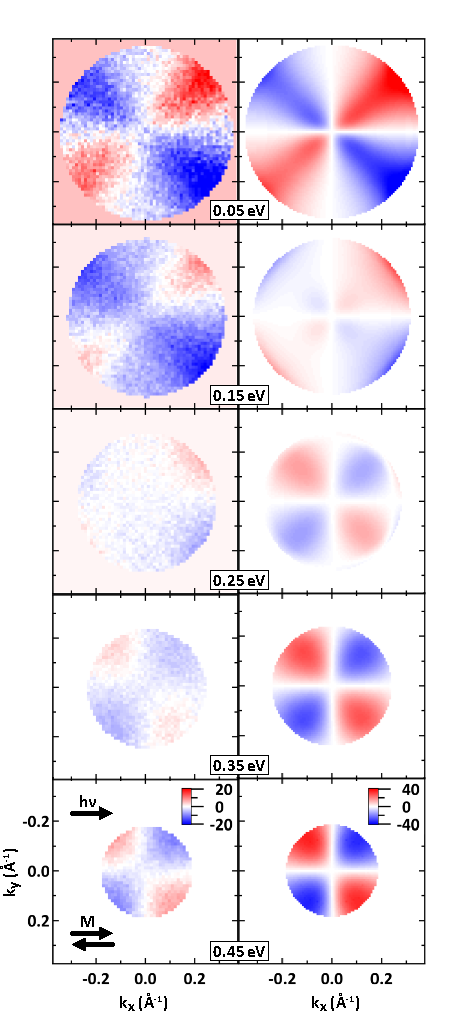
\includegraphics[width = 0.7\columnwidth]{FePaperApol.pdf}
    \caption{Momentum-resolved polarization asymmetry $A_{\mathrm{pol}}$ of Fe(001) at selected binding energies for 70° grazing light incidence. Right column: theoretical results obtained from photoemission calculations. The binding energy is indicated at each panel. The color scale, showing $A_{\mathrm{pol}}$ as defined in Eq.~\eqref{eq:Apol} in percent, is identical for all panels in this column. 
    Left column: respective experimental results. The arrow marked $h \nu$ indicates the light incidence direction. The arrows M represent the two magnetization directions considered for $A_{\mathrm{pol}}$. 
    % $\Gamma$ is the center of the surface Brillouin zone ($\vec{k}_{\parallel} = 0$).
    \todo[inline]{Details of figure (background) still in work}
    }
    \label{fig:Apol}
\end{figure}


\paragraph{Contrast mechanisms.} 
The polarization asymmetry $A_{\mathrm{pol}}$ as defined in Eq.~\eqref{eq:Apol} and depicted in Fig.~\ref{fig:Apol}, depends on the binding energy of the initial states. Both, theoretical (top row) and experimental data (bottom row), show that this contrast mechanism is sizable with absolute values up to about $\unit[40]{\%}$ in theory and $\unit[20]{\%}$ in experiment and thus cannot be ignored. 
The theoretical patterns (top row in Fig.~\ref{fig:Apol}) exhibit two nodal lines at $k_{x} = 0$ and at $k_{y} = 0$. Moreover, one finds changes of sign if either $k_{x}$ or $k_{y}$ is reversed. These features are imposed by the symmetry of the setup, specifically the off-normal light incidence. The experimental counterparts (bottom row) display the same features but slightly oblique or off-center, most clearly for binding energies with comparably small asymmetry (cf.\ $\unit[0.15]{eV}$ and $\unit[0.25]{eV}$). We attribute these deviations to imperfections in experiment, for example a small misalignment of the light incidence with respect to a crystal mirror plane. \rework{Moreover, we assume an electron self energy that is independent of $k_{\parallel}$ (see \cite{Supplement}).} Nevertheless, the agreement between experiment and theory is remarkable good over the full range of electron binding energies. Note that the experimental asymmetries have been determined from two separate 2D momentum maps for magnetization directions $+\vec{M}$ and $-\vec{M}$ with respect to the [100] direction via selection of appropriate single magnetic domains.

The energy-dependent exchange asymmetry $A_{\mathrm{ex}}$, defined in Eq.~\eqref{eq:Aex} and shown in Fig.~\ref{fig:Aex}, exhibits absolute values up to $\unit[10]{\%}$ in theory and $\unit[6]{\%}$ in experiment. It exhibits a clear odd symmetry upon reversal of $k_{x}$, whereas it does not change sign upon reversal of $k_{y}$, in contrast to $A_{\mathrm{pol}}$. Both features are dictated by the symmetry of the setup (see \cite{Supplement}), while the absolute value and the sign of the asymmetries depend on the initial state binding energy via the band structure and photoemission matrix elements.

The above findings support that the asymmetries $A_{\mathrm{pol}}$ and $A_{\mathrm{ex}}$ are suitable tools to disentangle and to quantify the main contrast mechanisms for domain imaging. 
\begin{figure}
    \centering
    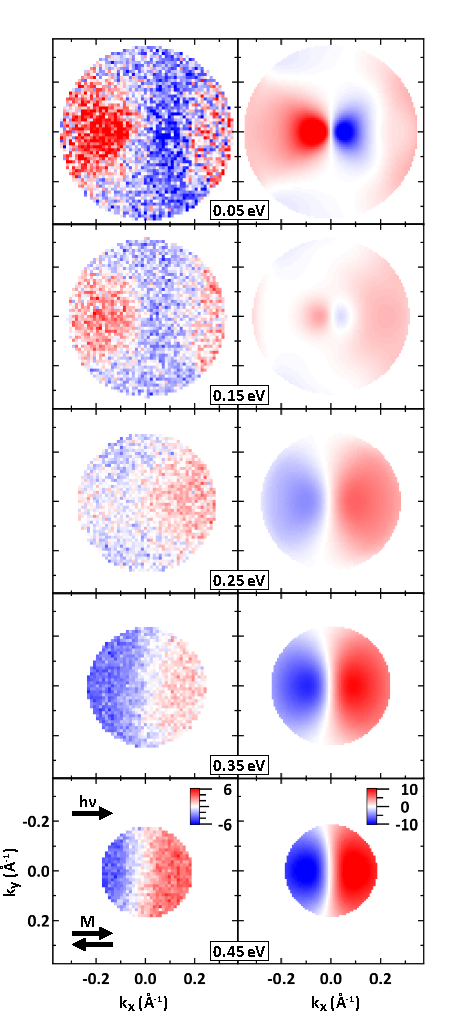
\includegraphics[width = 0.7\columnwidth]{FePaperAex.pdf}
    \caption{Momentum-resolved exchange asymmetry $A_{\mathrm{ex}}$ of Fe(001) at selected binding energies, as in Fig. \ref{fig:Apol}. Left column shows experimental PEEM data, whereas photoemission calculations are presented in the right column. Note that small differences with respect to an odd symmetry upon reversal of $k_{x}$ result from grazing light incidence. For normal incidence they are absent.}
    \label{fig:Aex}
\end{figure}


\paragraph{Domain imaging.} 

From the momentum-resolved $A_{\mathrm{ex}}$ pattern in Fig.~\ref{fig:Aex}, it follows directly that MCD imaging might reveal strong magnetic contrast in case of \textit{off-normal} electron momentum selection. On the other hand, different momentum contributions will largely cancel without momentum selection or with a momentum selection centered at $k_x=k_y=0$. The latter has been widely applied and explains small or vanishing magnetic dichroism for in-plane magnetic domains reported so far \cite{marx2000}.
\begin{figure}
    \centering
    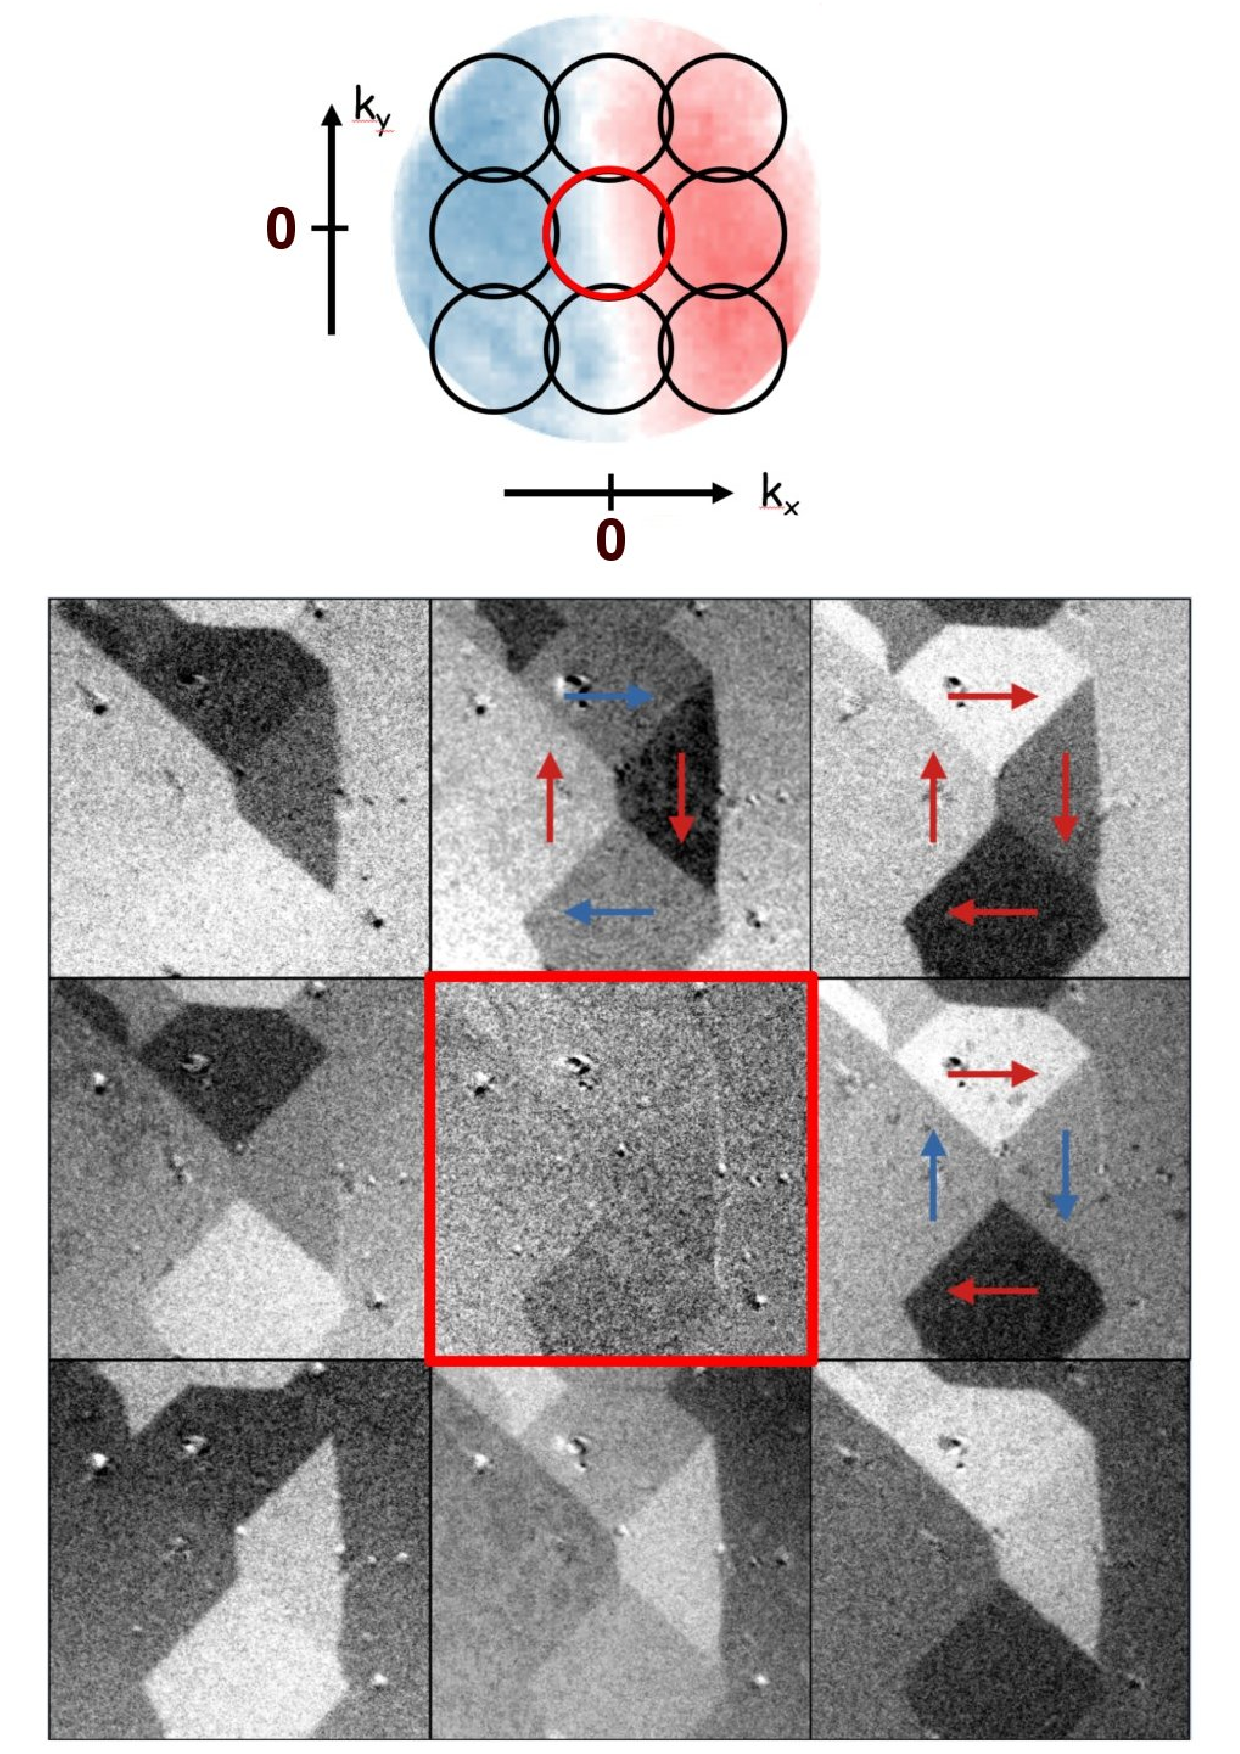
\includegraphics[width = 0.7\columnwidth]{Darkfield_overview.pdf}
    \caption{Darkfield MCD imaging of Fe(100). Top: Schematics of the nine aperture positions in the momentum plane (Momentum-resolved $A_{\mathrm{ex}}$ pattern set as background). Bottom: Domain imaging using the nine aperture positions shown above. Photon energy $\unit[5.2]{eV}$, grazing light incidence, \rework{binding energy $\unit[xx]{eV}$.}}
    \label{fig:Imaging}
\end{figure}

To enhance the magnetic contrast, we place a circular contrast aperture in a $\vec{k}_{\parallel}$ area of high exchange asymmetry: essentially reducing the area of interest in $\vec{k}_{\parallel}$ space to a "high-exchange" region. This procedure is known as dark-field imaging in optics. 
Figure \ref{fig:Imaging} (top) shows nine different contrast aperture positions as black circles in $\vec{k}_{\parallel}$ space, which result in nine corresponding MCD PEEM images of the same Fe(001) surface region (Fig. \ref{fig:Imaging}, bottom), which shows in the center a Landau-like pattern of four orthogonal magnetic domains. For the centred aperture marked in red, the MCD contrast almost vanishes. On the other hand, an aperture centered at $k_x > 0$ and $k_y=0$ results in a drastically increased contrast of $\unit[6]{\%}$ for magnetic domains oriented in +x versus -x direction, whereas the contrast for domains oriented in +y and -y directions (blue arrows) vanishes. Both observations match quantitatively the result of the $\vec{k}_{\parallel}$ space measurements in Fig. \ref{fig:Aex}(b). Moving the momentum aperture $k_x < 0$ and $k_y=0$, reverses the contrast of +x and -x domains. 
As expected, the contrast switches from sensitivity in x direction to y direction when positioning the aperture at $k_x = 0$ and $k_y > 0$ (upper-middle PEEM image in \ref{fig:Imaging}). The upper-right measurement shows a diagonal position with $k_x > 0$ and $k_y > 0$, where the different contributions to the MCD signal mix, resulting in four different asymmetry values for the four in-plane magnetization directions. 

\paragraph{Band structure effects.}
The size of $A_{\mathrm{ex}}$ and, therefore, the MCD contrast in PEEM for near-threshold photoemission depend on the initial state energy as is demonstrated in Fig.~\ref{fig:Aex}. $A_{\mathrm{ex}}$ reverses sign from about $\unit[+6]{\%}$ slightly below the Fermi level to $\unit[-6]{\%}$ at $E_B= 0.44\,eV$. 
% For larger binding energies, it decreases again with an absolute value below $\unit[1]{\%}$ at $\unit[0.65]{eV}$. 
These momentum- and energy-resolved PEEM data have been crosschecked with higher energy resolution in a second, angle-resolved photoelectron spectroscopy (ARPES) setup described elsewhere \cite{gillmeister2018, gillmeister2020} for an oxygen-passivated Fe(001) thin film and depicted in Fig.~\ref{fig:AexContrast} (a). The maximum $A_{\mathrm{ex}}$ values as determined by PEEM for oxygen-passivated Fe(001) are displayed in Fig.~\ref{fig:AexContrast} (b) for comparison. Again, both experiments reveal a maximum value of $A_{\mathrm{ex}}$ at the Fermi level, as well as a sign change and a negative maximum at 0.16 and $\unit[0.44]{eV}$, respectively, with a decreasing value for lower binding energies. Note that this observation calls for exact threshold photoexcitation or for an energy-resolved electron detection in order to obtain high MCD signals. Otherwise the positive and negative exchange asymmetries will partly cancel each other.

While the darkfield scheme of threshold MCD PEEM is broadly applicable, the magnitude of the binding-energy dependent exchange asymmetry $A_{\mathrm{ex}}$ is a material-specific property. It results from the spin-dependent band structure of Fe(001) and the corresponding photoemission matrix elements. Note that these matrix elements are photon energy dependent due to the selection of different photoemission final states.

\begin{figure}
    \centering
    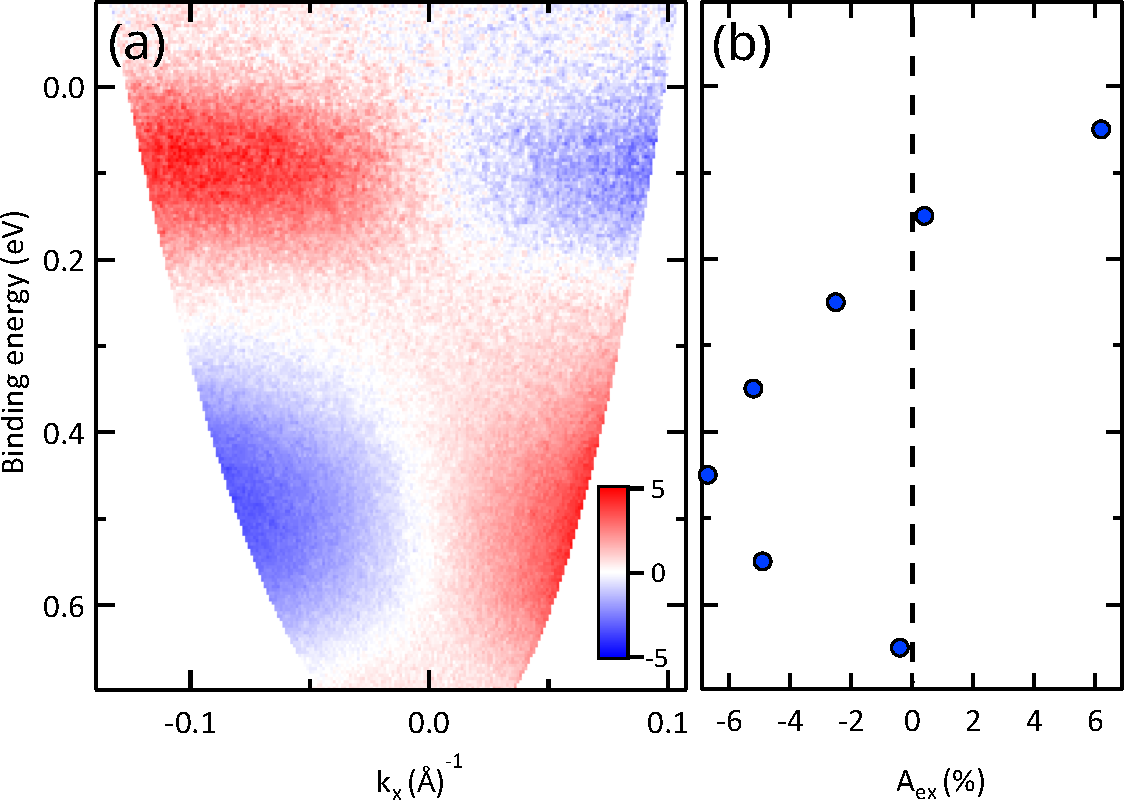
\includegraphics[width = 0.9\columnwidth]{Fe001-O_2.pdf}
    \caption{Binding-energy dependent exchange asymmetry $A_{\mathrm{ex}}$ for Fe(001)-(1x1)-O at $h\nu = 5.2\,eV$. (a) ARPES data for an oxygen-passivated Fe(001) thin film grown on MgO(001) with sample magnetized in +x and -x direction (light incidence at 70°, $k_y = 0$). (b) Momentum-selected PEEM data for an oxygen-passivated Fe(001) single crystal (\rework{selection at $k_x = \unit[xx]{\AA}$, $k_y = 0$}, light incidence at 60°). \todo[inline]{Check signs in figure}
    }
    \label{fig:AexContrast}
\end{figure}

\paragraph{Summary and prospects.} The present investigation proves that magnetic domains can be imaged with high contrast with threshold PEEM using a momentum-selection of the detected photoelectrons as concept of darkfield threshold MCD PEEM. 

For a proof-of-principle, we applied darkfield UV PEEM to an in-plane magnetized Fe(001) surface. However, the approach is general so that it can easily be applied to other ferromagnets, even to those with include out-of-plane magnetization \cite{kronseder2011}. Thus, it is well suited for studying magnetic reorientation transitions, as for example observed for Ni/Cu(001) \cite{fukumoto2002,sander2004,nakagawa2006,kronseder2011}. We see its main capabilities, however, in investigations of ultrafast magnetization dynamics using femtosecond laser pulses in a optical pump and threshold UV photoemission probe scheme. For applications it paves the way for imaging the ultrafast motion of domain walls \cite{parkin2008} or of large skyrmions on nanometer lengthscales \cite{goebel2019,jani2021,kern2022}.

\paragraph{Acknowledgments.} This work is funded by the Deutsche Forschungsgemeinschaft (DFG, German Research Foundation) -- Project-ID 328545488 -- TRR~227, projects~A06 and~B04.

% \bibliographystyle{}
\bibliography{references}

\listoftodos

\end{document}
